\documentclass{beamer}
\mode<presentation> {
    \usetheme{CambridgeUS}
    \usecolortheme{dolphin}
}
\setbeamercolor*{title}{use=structure,fg=white,bg=structure.fg}

\setbeamertemplate{section in toc}{\color{structure}\inserttocsectionnumber.\color{black}~\inserttocsection\par}
\setbeamertemplate{subsection in toc}{\color{structure}~~\inserttocsectionnumber.\inserttocsubsectionnumber.\color{black}~\inserttocsubsection\par}
\setbeamertemplate{itemize items}[default]
\setbeamertemplate{enumerate items}[default]

\setbeamertemplate{bibliography entry title}{}
\setbeamertemplate{bibliography entry location}{}
\setbeamertemplate{bibliography entry note}{}

\usepackage[latin1]{inputenc}
\usepackage{lmodern}
\usepackage{graphicx}
\usepackage{eurosym}
\usepackage{media9}
\usepackage{tikz}
\usepackage{url}
\usepackage{hyperref}

%----------------------------------------------------------------------------------------------------------------------

\title[Robobo Line Follower]{Robobo Line Following Program with ROS}
\author{\^Angela Cardoso}
\institute[MIEIC - FEUP]{Master in Informatics and Computing Engineering \\
    \smallskip
    Faculty of Engineering of the University of Porto \\
}

\date{\today} 

\begin{document}

%----------------------------------------------------------------------------------------------------------------------

%%%%%%%%%%%%%%
% TITLE PAGE %
%%%%%%%%%%%%%%
\begin{frame}
\titlepage
\end{frame}

%----------------------------------------------------------------------------------------------------------------------

%%%%%%%%%%%%
% OVERVIEW %
%%%%%%%%%%%%
\begin{frame}
\frametitle{Overview} 
\small
\tableofcontents
\end{frame}

%----------------------------------------------------------------------------------------------------------------------

%%%%%%%%%%
% ROBOBO %
%%%%%%%%%%
\section{Introduction} 
\subsection{Robobo} 
\begin{frame}
\frametitle{Robobo}
\begin{minipage}[t]{.34\textwidth}
\begin{center}
%\vspace{0.5cm}
\includegraphics[scale=0.5]<+->{img/robobo.png}
\end{center}
\end{minipage}
\hfill
\begin{minipage}[t]{.62\textwidth}
\vspace{-0.2cm}
\begin{itemize}[<+->]
	\item Developed by Mytechia
    \item Two wheels and a plastic caster
    \item 8 infrared sensors and 7 LEDs
    \item Phone holder with pan and tilt movements
    \item Phone connects to base via Bluetooth
    \item Phone connects to computer via Wi-Fi
    \item Phone sensors: cameras, gyroscope, accelerometer
    \item Phone actuators: display, sound
    \item Programmable using ScratchX, Java and ROS
\end{itemize}
\end{minipage}
\end{frame}

%----------------------------------------------------------------------------------------------------------------------

%%%%%%%%%%%%%%%%
% ARCHITECTURE %
%%%%%%%%%%%%%%%%
\section{Architecture} 
\subsection{Maps} 
\begin{frame}
\frametitle{Maps}
\begin{center}
\includegraphics[scale=0.08]<+>{img/map_black.png}
\includegraphics[scale=0.08]<+>{img/map_color_final.jpg}
\end{center}
\end{frame}

%----------------------------------------------------------------------------------------------------------------------

\subsection{Behavior} 
\begin{frame}
\frametitle{Behavior}
\begin{center}
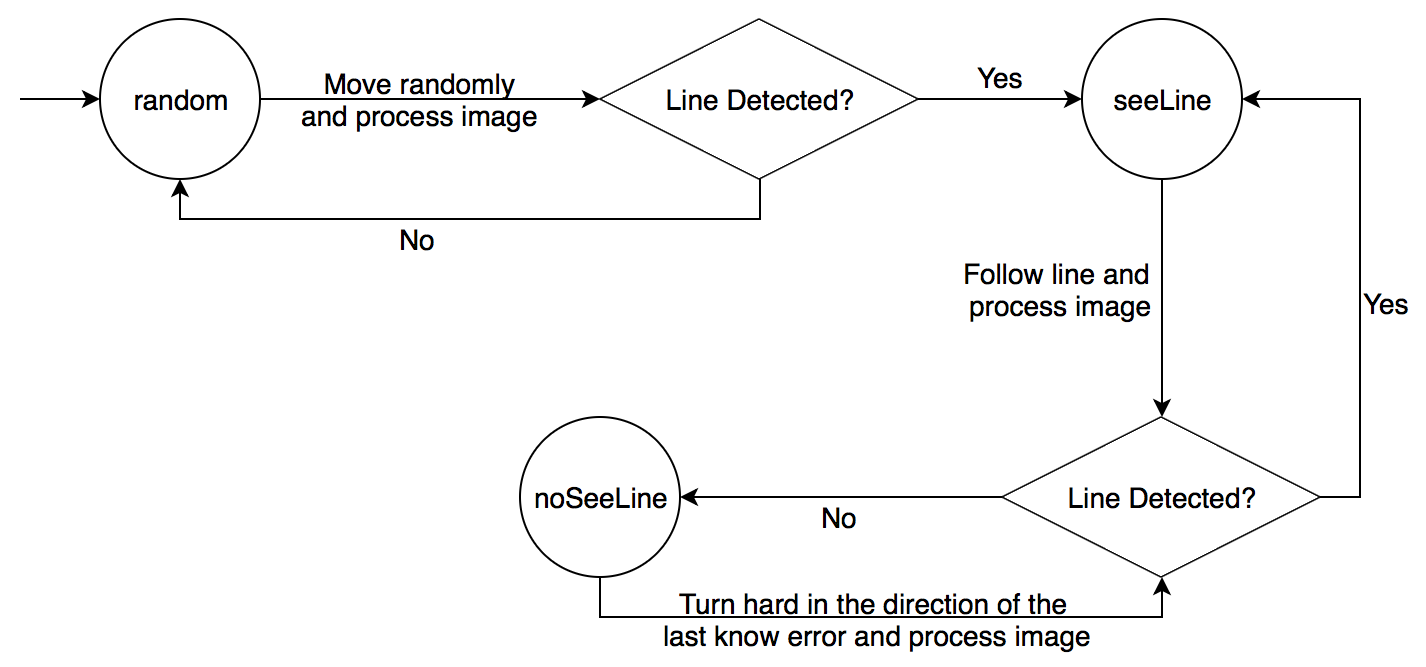
\includegraphics[scale=0.45]{img/architecture.png}
\end{center}
\end{frame}

%----------------------------------------------------------------------------------------------------------------------

\subsection{Algorithms} 
\begin{frame}
\frametitle{Camera Image Processing}
\begin{enumerate}
	\item<1-> Receive camera image
	\begin{center}
	\includegraphics[scale=0.3]<1>{img/image.png}
	\end{center}
	\vspace{-0.65cm}
	\item<2-> Select Region Of Interest (ROI)
	\begin{center}
	\includegraphics[scale=0.3]<2>{img/roi.png}
	\end{center}
	\vspace{-0.65cm}
	\item<3-> Create mask where only the color the robot should follow is selected
	\item<3-> Make all pixels that do not belong to the mask white
	\begin{center}
	\includegraphics[scale=0.3]<3>{img/mask.png}
	\end{center}
	\vspace{-0.65cm}
	\item<4-> Transform the ROI from color to gray scale
	\begin{center}
	\includegraphics[scale=0.3]<4>{img/mono.png}
	\end{center}
	\vspace{-0.65cm}
	\item<5-> Blur the gray scale ROI
	\begin{center}
	\includegraphics[scale=0.3]<5>{img/blur.png}
	\end{center}
	\vspace{-0.65cm}
	\item<6-> Compute threshold of blurred ROI
	\begin{center}
	\includegraphics[scale=0.3]<6>{img/thresh.png}
	\end{center}
	\vspace{-0.65cm}
	\item<7-> Find contours and select the contour closest to the center
	\begin{center}
	\includegraphics[scale=0.3]<7>{img/contour.png}
	\end{center}
	\vspace{-0.65cm}
	\item<8-> Compute the centroid of that contour using image moments
	\begin{center}
	\includegraphics[scale=0.3]<8>{img/centroid.png}
	\end{center}
	\vspace{-0.65cm}
	\item<9-> Use the centroid to determine the signed normalized error
\end{enumerate}

\end{frame}

%----------------------------------------------------------------------------------------------------------------------

\begin{frame}
\frametitle{Line Following}
\begin{enumerate}[<+->]
	\item Compute angular velocity using a PID controller:
		$$\omega = K_p * P + K_i * I + K_d * D,$$
		$K_p, K_i, K_d$: proportional, integral and derivative constants

		$P, I, D$: proportional, integral and derivative terms
		
		$P = e, I = I + e, D = e - d$: $e$ current error, $d$ previous error
	\item Send move command to each wheel, with left wheel speed $v - \omega$ and right wheel speed $v + \omega$, for a linear velocity $v$.
	\item After tunning, the constants used where~$K_p = 8, K_i = 0, K_d = 8$, with a linear velocity of~$8$.
\end{enumerate}
\end{frame}

%----------------------------------------------------------------------------------------------------------------------

%%%%%%%%%%%
% RESULTS %
%%%%%%%%%%%
\section{Results}
\subsection{Black Map} 
\begin{frame}
\frametitle{Black Map with Pencil}
\begin{center}
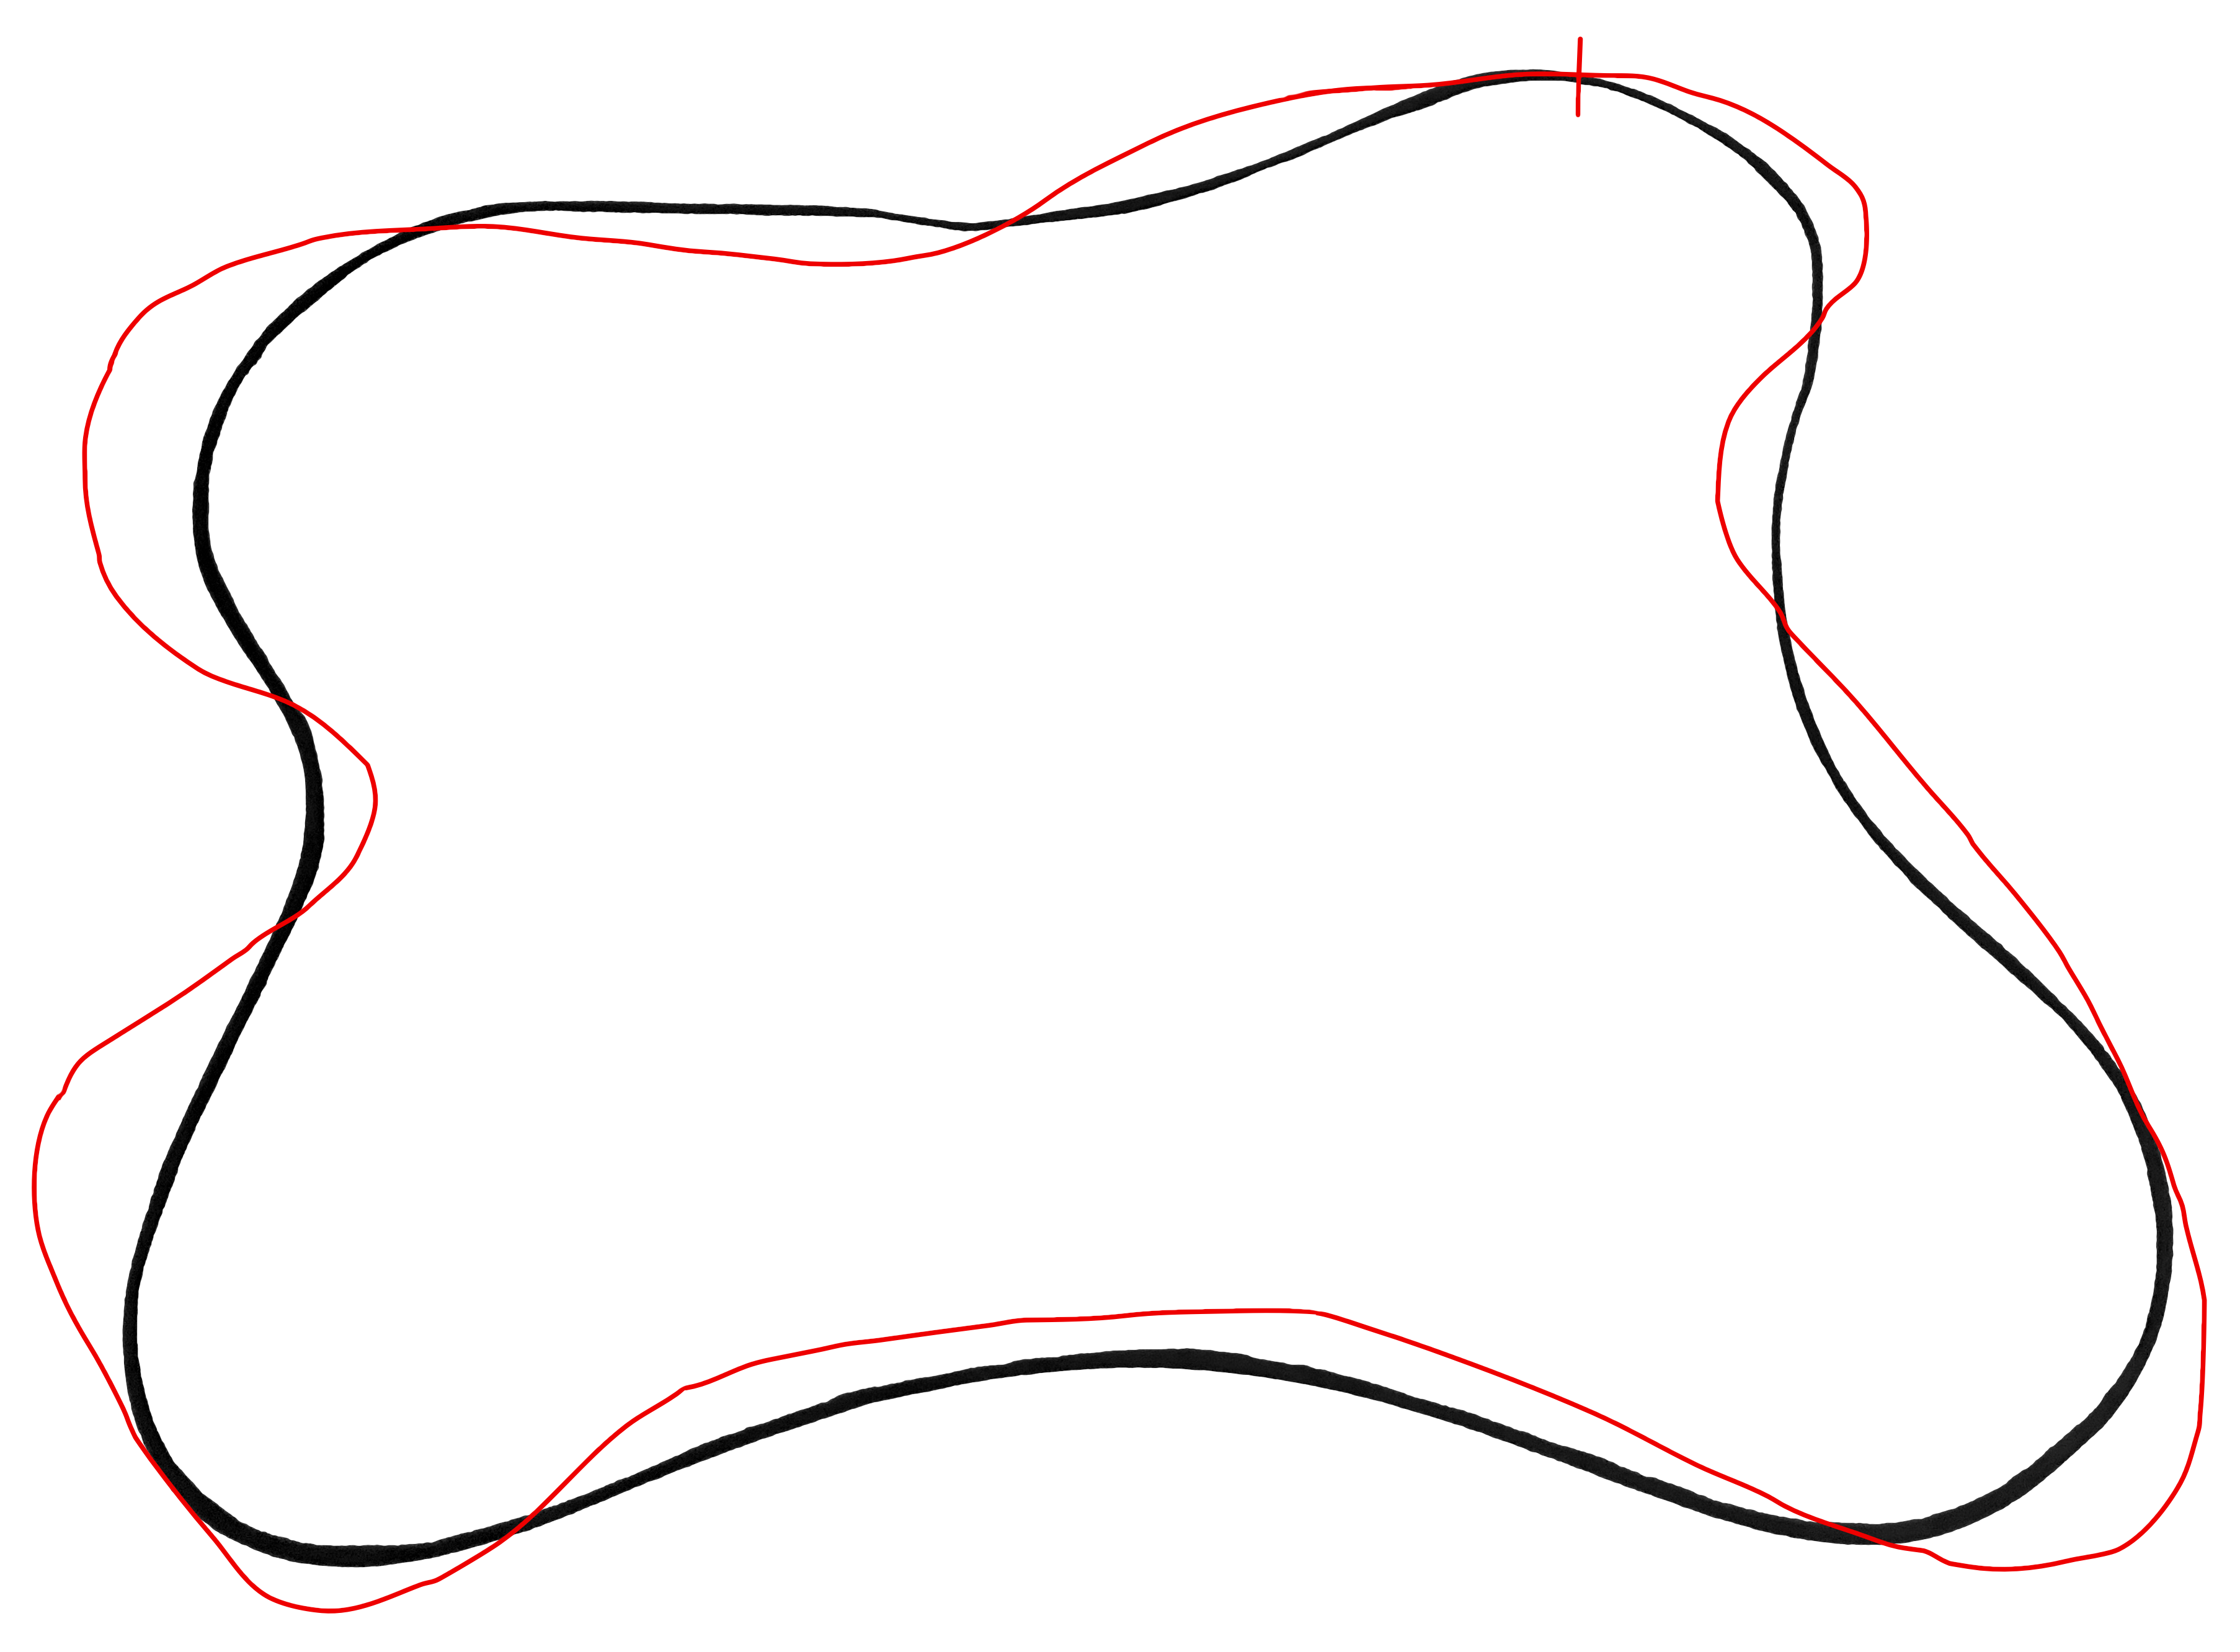
\includegraphics[scale=0.08]{img/result.png}
\end{center}
\end{frame}

%----------------------------------------------------------------------------------------------------------------------

\subsection{Colored Map} 
\begin{frame}
\frametitle{Colored Map Video}
\begin{center}
\href{run:video/robobo_line_follower.mp4}{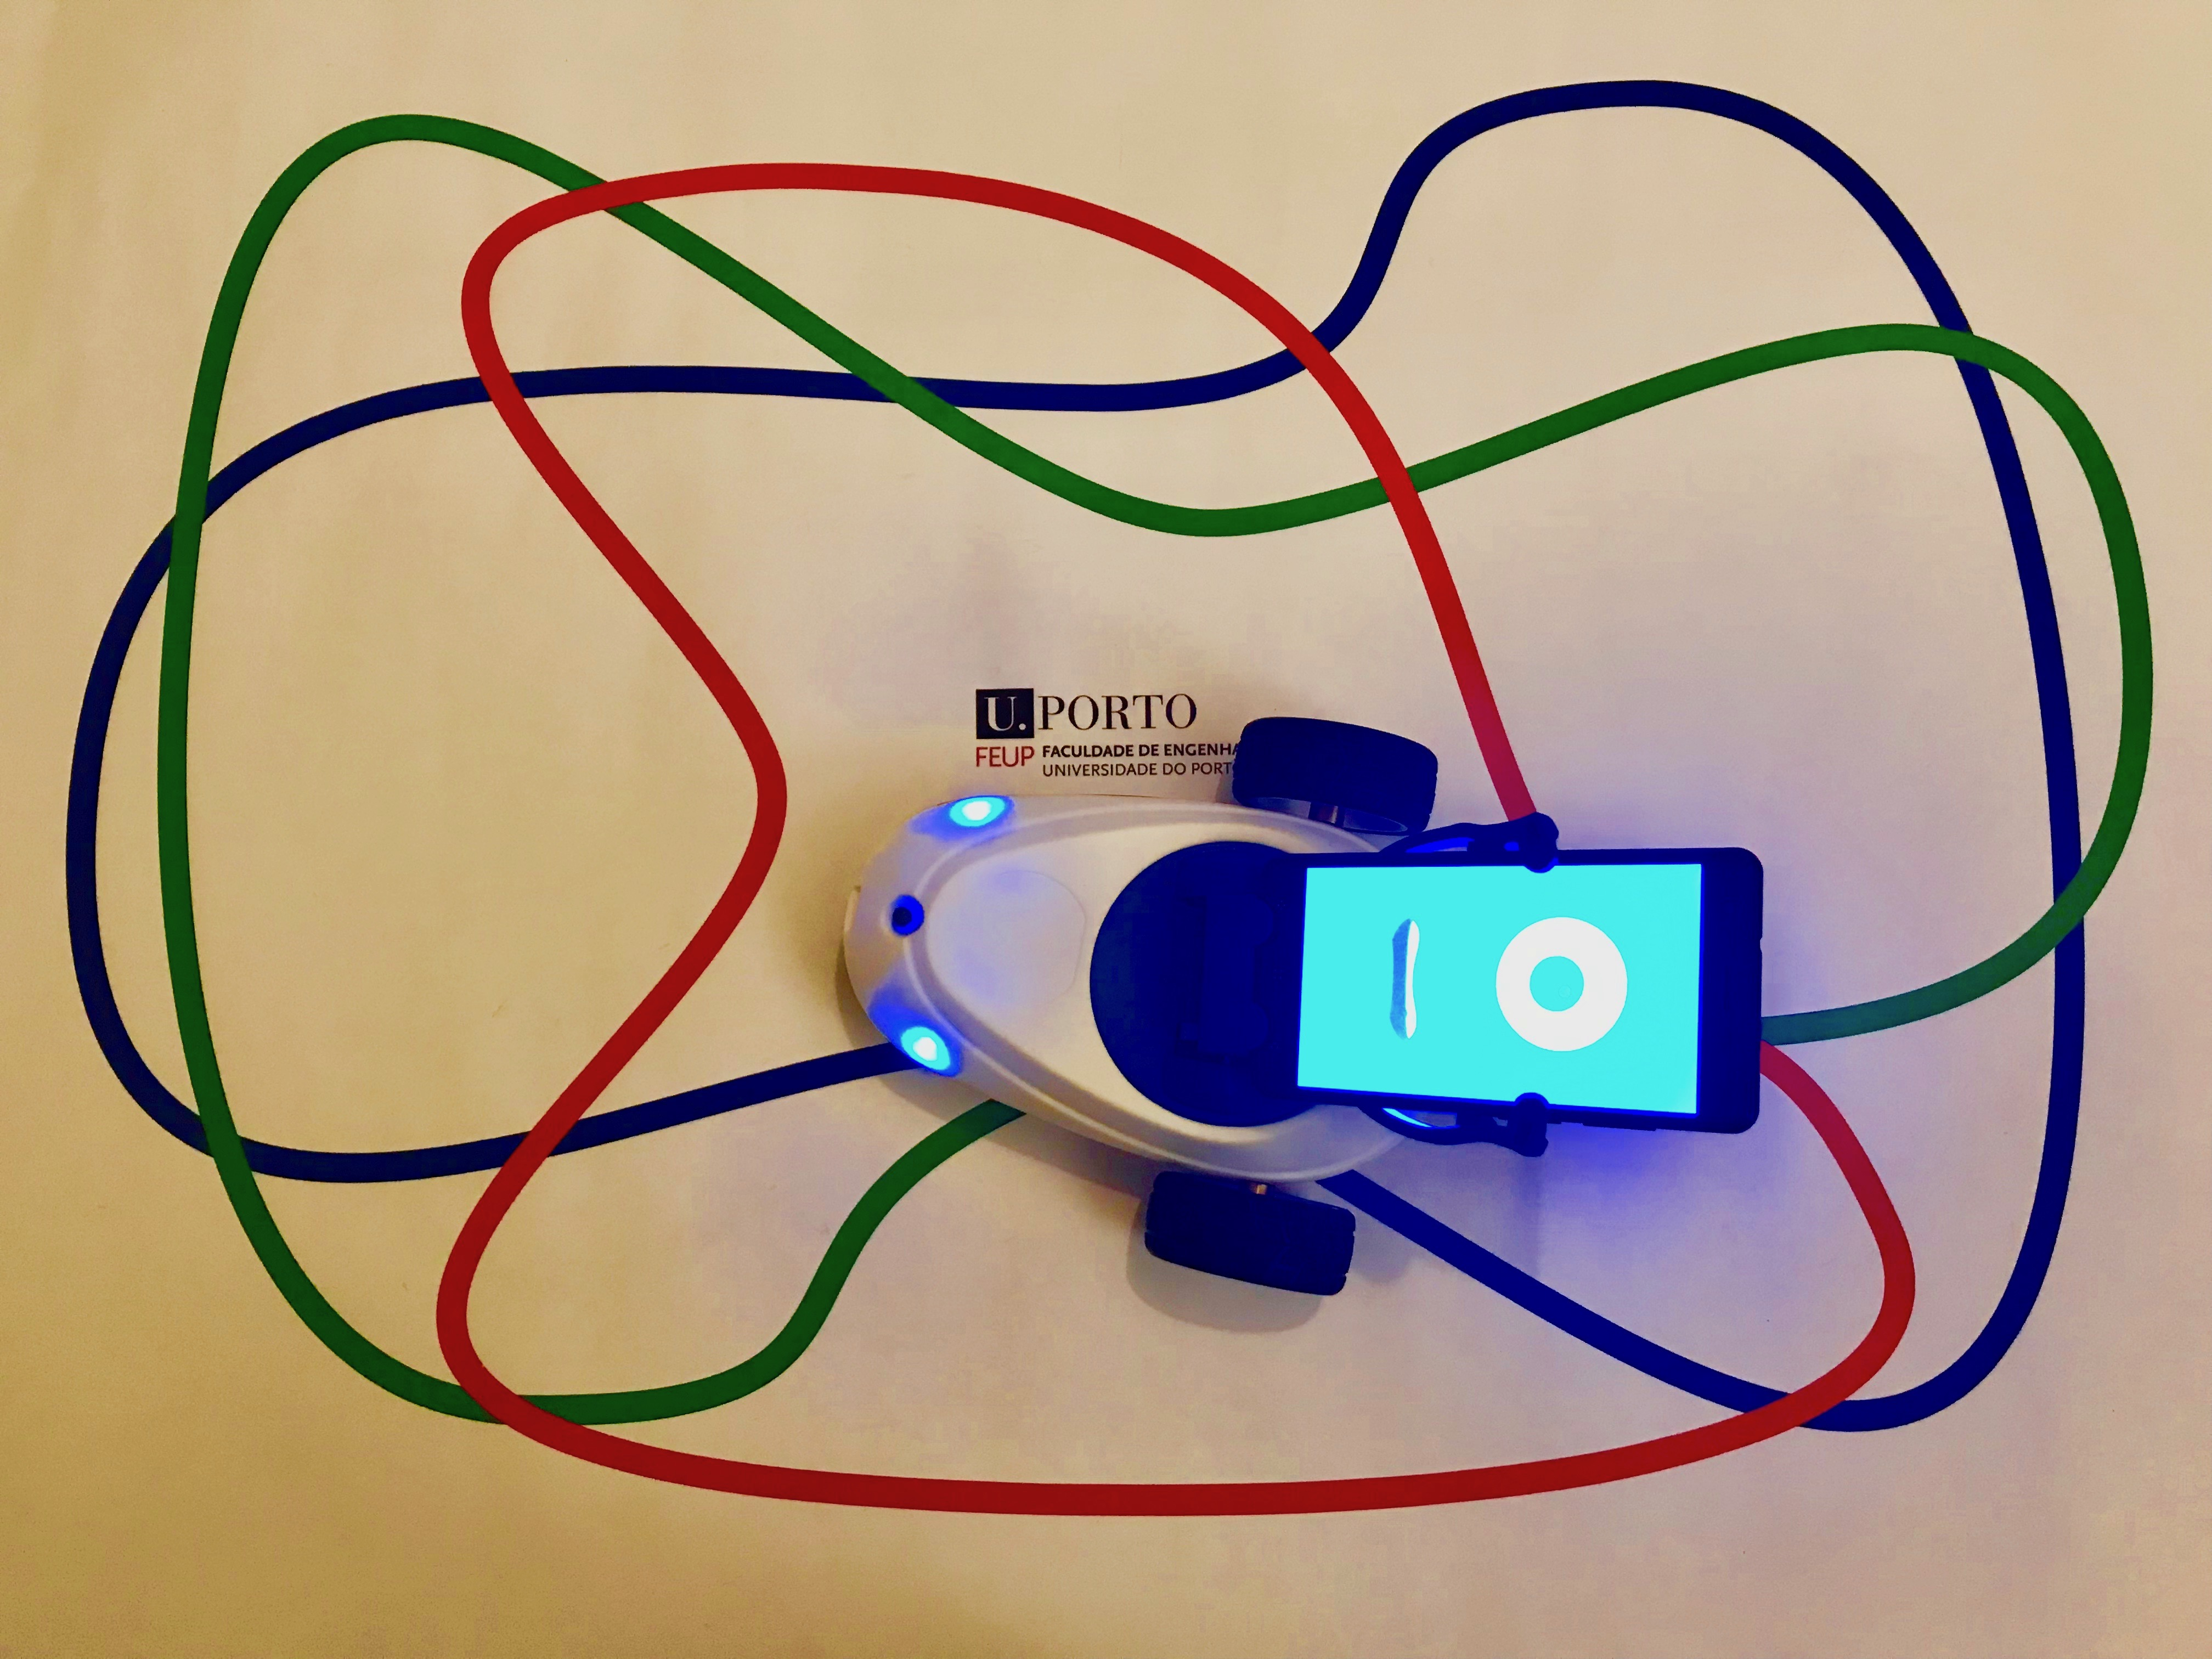
\includegraphics[scale=0.06]{img/map_color_robobo.jpg}}
\end{center}
\end{frame}

%----------------------------------------------------------------------------------------------------------------------

%%%%%%%%%%%%%%%
% LIMITATIONS %
%%%%%%%%%%%%%%%
\section{Limitations}
\begin{frame}
\frametitle{Limitations}
\begin{itemize}[<+->]
	\item Initial robot position
    \item Camera image width
    \item Linear velocity
\end{itemize}
\end{frame}

%----------------------------------------------------------------------------------------------------------------------

%%%%%%%%%%%%%%
% CONCLUSION %
%%%%%%%%%%%%%%
\section{Conclusion}
\begin{frame}
\frametitle{Conclusion}
\begin{itemize}[<+->]
	\item The PID controller, although hard to tune provides a stable movement
	\item The camera image processing is the most challenging, but also the most rewarding part
    \item For real world projects, sometimes one must use tricks to overcome some of the limitations
    \item Using ROS to program Robobo is pretty much the same as programming any other robot
\end{itemize}
\end{frame}

%----------------------------------------------------------------------------------------------------------------------

%%%%%%%%%%%%%%%%
% BIBLIOGRAPHY %
%%%%%%%%%%%%%%%%
\section{Bibliography}
\begin{frame}
\frametitle{Bibliography}
	{\scriptsize
		\bibliographystyle{abbrv}
		\nocite{*}
    	\bibliography{line_bib}
    }
\end{frame}

\end{document} 
